\documentclass[aspectratio=169,11pt]{beamer}
\usetheme{Copenhagen}      % layout: split headline w/ section+subsection tabs
\usecolortheme{beaver}     % palette: dark red + gray on white
\setbeamertemplate{navigation symbols}{}
\usepackage{graphicx}
\usepackage{booktabs}
\usepackage{amssymb}
\usepackage{xcolor}
\usepackage{tikz}
\usetikzlibrary{arrows.meta,positioning}
\definecolor{accent}{HTML}{2A4D7A}
\definecolor{warn}{HTML}{B23A1E}
\definecolor{good}{HTML}{2E7D32}
\setbeamercolor{frametitle}{fg=accent}
\setbeamercolor{title}{fg=accent}
\setbeamercolor{structure}{fg=accent}
\setbeamerfont{frametitle}{series=\bfseries}
\setbeamertemplate{itemize items}[circle]
\setbeamertemplate{footline}[frame number]
\newcommand{\tc}[1]{\texttt{#1}}
\newcommand{\term}[1]{\textbf{#1}}
\newcommand{\bert}[1]{\textbf{BERT\,#1}}
\newcommand{\y}{\textcolor{good}{\checkmark}}
\newcommand{\n}{\textcolor{warn}{\ensuremath{\times}}}
\newcommand{\todo}{\textcolor{warn}{\textbf{TODO}}}
\newcommand{\cbar}[1]{\textcolor{accent}{\rule{#1}{5pt}}}

\title{\textbf{Quality Control for Synthetic Biomedical Relation Data}}
\subtitle{Midterm presentation}
\author{Hamed Feizabadi \and Christoph Geron}
\institute{MA-INF 4237 NLP Lab, CAISA Lab \quad(supervisor: Frederik Labont\'e)}
\date{July 2026}

\begin{document}

\begin{frame}[plain]\titlepage\end{frame}

% ---------------------------------------------------------------- problem
\begin{frame}{The problem, and the idea}
  \textbf{Problem.} Biomedical relation extractors need labelled data, but expert
  datasets are tiny. Synthetic abstracts from an LLM are cheap, but we cannot trust
  the LLM actually wrote the relations we asked for.
  \vspace{0.4em}
  \begin{itemize}
    \item \textbf{The idea:} a \term{quality-control (QC) filter} that reads a claimed
          relation triple + an abstract and says \emph{supported} / \emph{not}.
          Keep the good synthetic examples, drop the bad.
    \item Two models: \bert{1} (relation classifier, Chris) and \bert{2}
          (the QC filter, Hamed). Both small encoders (PubMedBERT), not LLMs.
  \end{itemize}
  \vspace{0.3em}
  \begin{center}
  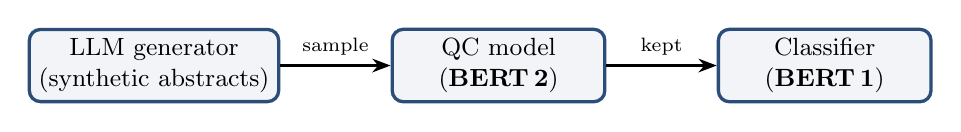
\begin{tikzpicture}[node distance=1.0cm and 1.4cm,>=Stealth,
    box/.style={draw=accent,very thick,rounded corners,minimum width=2.7cm,minimum height=0.9cm,align=center,fill=accent!6,font=\small}]
    \node[box] (llm){LLM generator\\(synthetic abstracts)};
    \node[box,right=of llm] (qc){QC model\\(\bert{2})};
    \node[box,right=of qc] (clf){Classifier\\(\bert{1})};
    \draw[->,thick] (llm)--node[above,font=\scriptsize]{sample}(qc);
    \draw[->,thick] (qc)--node[above,font=\scriptsize]{kept}(clf);
  \end{tikzpicture}
  \end{center}
\end{frame}

% ---------------------------------------------------------------- dataset
\begin{frame}{The dataset: perturbed BioRED}
  We build QC training data from real BioRED relations. A gold relation is a
  positive; controlled corruptions are negatives. Four classes: \tc{Association},
  \tc{Positive\_Correlation}, \tc{Negative\_Correlation}, \tc{NoRelation}.
  \begin{columns}[T]
    \begin{column}{0.52\textwidth}
      \small
      \begin{itemize}
        \item \tc{label\_flip}: wrong relation label (full 4$\times$4 matrix)
        \item \tc{direction\_swap}: reversed order (Pos/Neg only)
        \item \tc{fp\_external}: entity not in the abstract
      \end{itemize}
      \vspace{0.3em}
      Train 54{,}424 rows, seed 42, byte-reproducible, label-1 $\approx$15\%.
      {\small\itshape (run 2 resamples this for training: see slide 8.)}
    \end{column}
    \begin{column}{0.48\textwidth}
      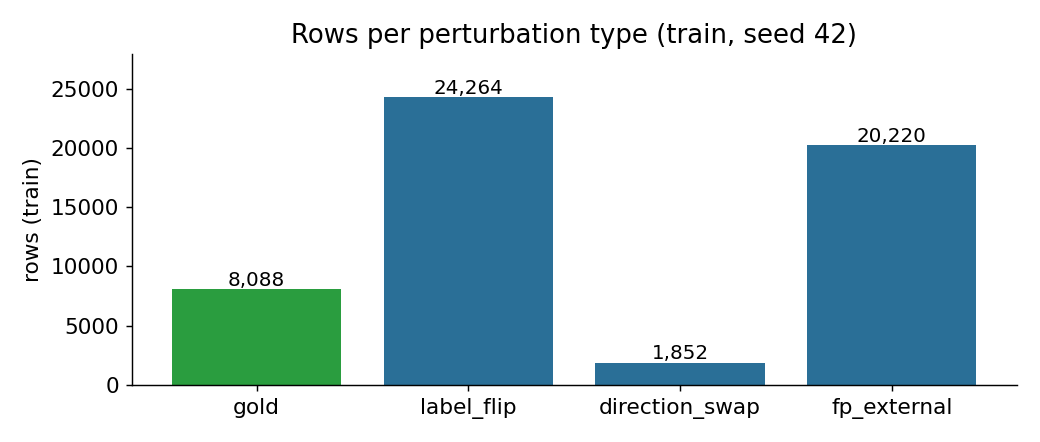
\includegraphics[width=\linewidth]{figures/01_rows_per_perturbation.png}
    \end{column}
  \end{columns}
\end{frame}

% ---------------------------------------------------------------- 4x4
\begin{frame}{\tc{label\_flip} over the full 4$\times$4 matrix}
  Every off-diagonal flip is a negative, including specific $\to$ \tc{Association}
  (the LLM may soften a correlation to association-level wording).
  \vspace{0.4em}
  \begin{center}
  \begin{tabular}{l|cccc|c}
    \toprule
    gold $\downarrow$ & As & Po & Ne & NoR & \# valid\\
    \midrule
    \tc{Association}          & -- & \y & \y & \y & 3\\
    \tc{Positive\_Correlation} & \y & -- & \y & \y & 3\\
    \tc{Negative\_Correlation} & \y & \y & -- & \y & 3\\
    \tc{NoRelation}           & \y & \y & \y & -- & 3\\
    \bottomrule
  \end{tabular}
  \end{center}
  \vspace{0.3em}
  {\small The \tc{$\to$NoR} column drops a real relation; the \tc{NoR$\to$} row claims
  one that is not there; specific $\to$ \tc{Association} weakens the label. All are
  mistakes the QC model must catch.}
\end{frame}

% ---------------------------------------------------------------- norelation
\begin{frame}{\tc{NoRelation}: distance-matched negatives}
  Co-mentioned non-pairs outnumber real relations $\approx$6.6:1 and sit farther
  apart. Sampling them raw teaches ``far apart $=$ no relation''. We distance-match
  (by \textbf{sentence gap}) and cap them.
  \begin{center}
    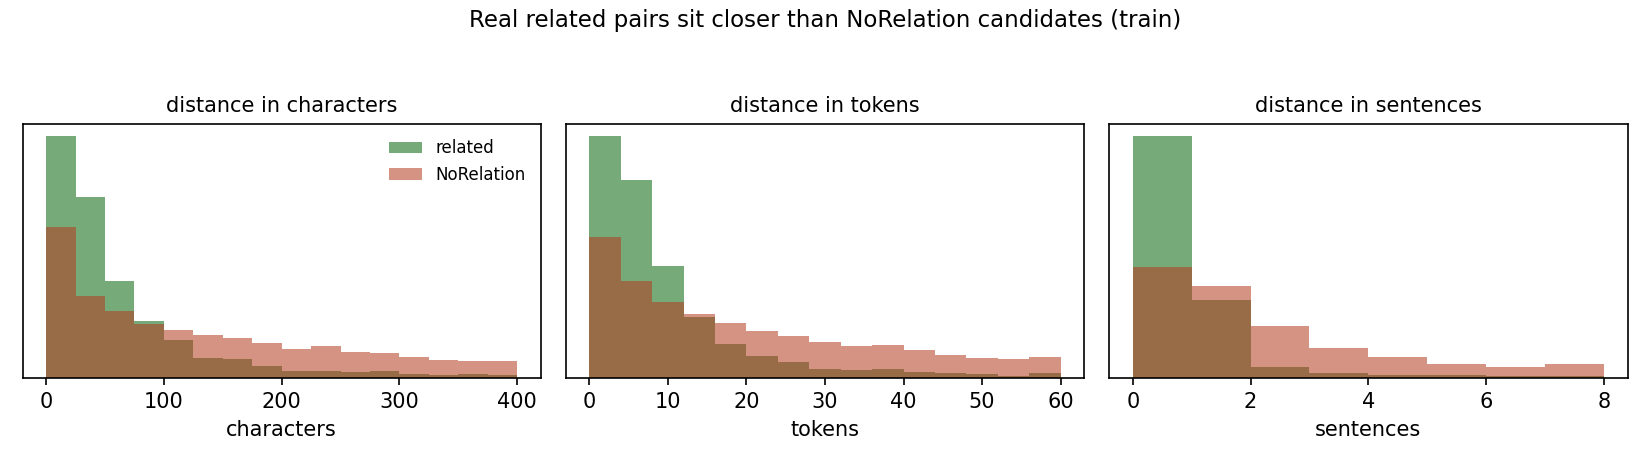
\includegraphics[width=0.86\textwidth]{figures/norel_distance.png}
  \end{center}
  {\small Real related pairs (green) are usually in the same sentence; \tc{NoRelation}
  pairs (red) are a sentence or more apart.}
\end{frame}

% ---------------------------------------------------------------- QC model
\begin{frame}{The QC model (\bert{2})}
  \begin{itemize}
    \item \textbf{Task:} claimed triple + abstract $\to$ supported (1) / unsupported (0).
    \item \textbf{Prompt:} \tc{Relation: A -> rel -> B} then \tc{Context: <abstract>}.
    \item \textbf{Model:} PubMedBERT, binary head.
    \item \textbf{Objective: precision, not F1} (synthetic data is cheap, so a strict
          filter is what we want).
  \end{itemize}
  \vspace{0.5em}
  {\small Two evaluations: intrinsic (does it work on the test set) and extrinsic
  (does filtering help \bert{1}).}
\end{frame}

% ---------------------------------------------------------------- run 1
\begin{frame}{Run 1: the pipeline works, but ...}
  \begin{columns}[T]
    \begin{column}{0.55\textwidth}
      First PubMedBERT run, test set:
      \begin{itemize}
        \item @0.5: precision \textbf{0.87}, recall \textbf{0.51}, F1 0.64
        \item precision-first threshold: precision 0.97, recall 0.28
      \end{itemize}
      \vspace{0.4em}
      \textbf{The catch:} recall 0.51. The data is $\approx$15\% positive / 85\%
      negative, so the model has little incentive to accept real relations. It was
      leaning toward ``no relation''.
    \end{column}
    \begin{column}{0.45\textwidth}
      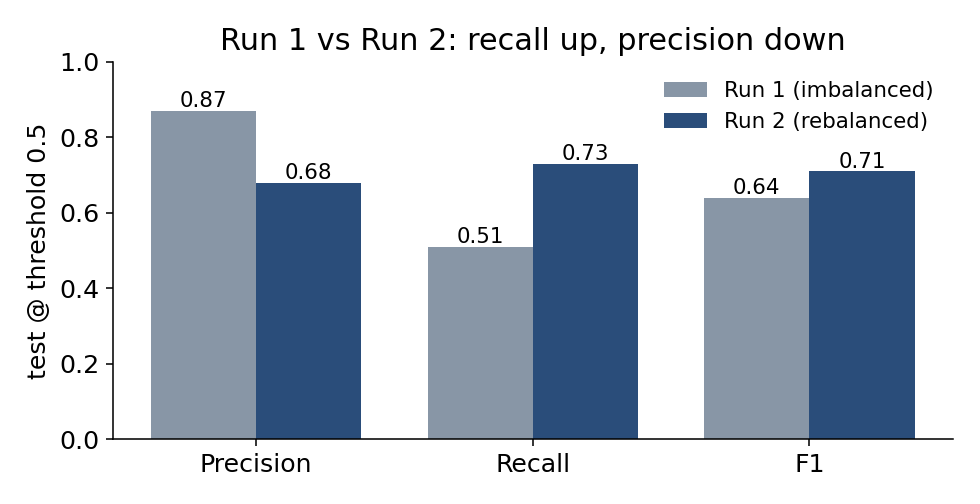
\includegraphics[width=\linewidth]{figures/run1_vs_run2.png}
    \end{column}
  \end{columns}
\end{frame}

% ---------------------------------------------------------------- run 2
\begin{frame}{Run 2: fixing the imbalance}
  \textbf{Fix (training only):} reduce \tc{fp\_external} to 25\% and duplicate the
  positive (gold) rows. Positive share 15\% $\to$ 34\%. Result: recall
  \textbf{0.51 $\to$ 0.73}, precision 0.87 $\to$ 0.68, F1 0.64 $\to$ 0.71; no longer
  just predicting ``no''.
  \begin{center}
    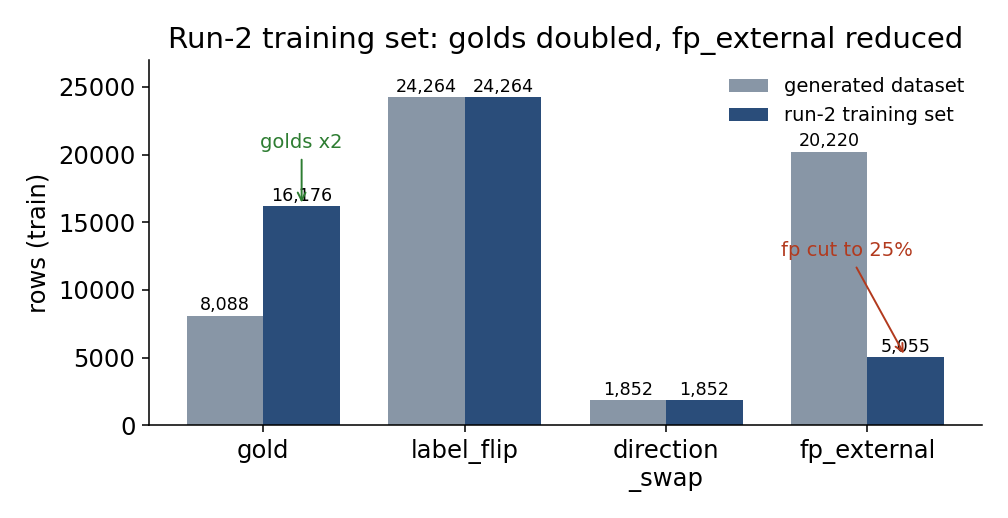
\includegraphics[width=0.74\textwidth]{figures/training_composition.png}
  \end{center}
\end{frame}

% ---------------------------------------------------------------- diagnosis
\begin{frame}{Diagnosis: real relations are the hard part}
  \begin{columns}[T]
    \begin{column}{0.5\textwidth}
      Gold recall broken down by the claimed relation type. The model accepts
      \tc{NoRelation} claims easily, but the real relations lag. It is learning them
      now ($\approx$55\%), just not as well.
    \end{column}
    \begin{column}{0.5\textwidth}
      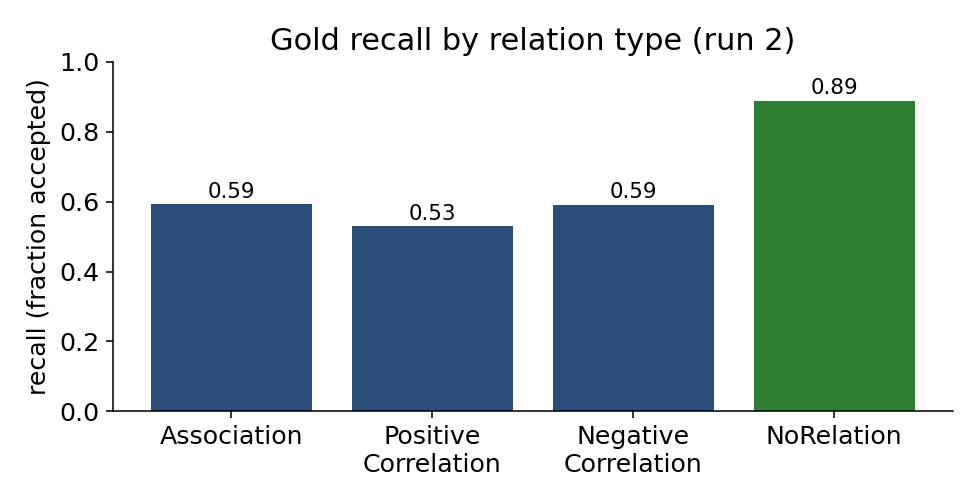
\includegraphics[width=\linewidth]{figures/gold_recall_by_type.png}
    \end{column}
  \end{columns}
\end{frame}

% ---------------------------------------------------------------- abstract level
\begin{frame}{Abstract-level evaluation}
  The filter judges a \emph{whole abstract}, not one pair: reject the abstract if
  $\ge N$ of its relations are flagged as wrong.
  \begin{columns}[T]
    \begin{column}{0.48\textwidth}
      \small
      Two kinds of abstract:
      \begin{itemize}
        \item \textbf{correct} = every relation in it is right (a clean synthetic
              abstract) $\to$ we want to \emph{keep} it.
        \item \textbf{faulty} = it has a wrong relation (we simulate: a correct
              abstract + 1 injected wrong one) $\to$ we want to \emph{catch} it.
      \end{itemize}
      \vspace{0.2em}
      Strict (\tc{$\ge$1}): catches every faulty abstract, but keeps only \textbf{19\%}
      of correct ones ($\approx$7 relations each, so false-rejections compound).
      Loosening keeps more correct but catches fewer faulty.
      \vspace{0.2em}

      Supervisor: keeping only 19\% is fine \emph{if almost no faulty one slips
      through}. Lever = higher recall.
    \end{column}
    \begin{column}{0.52\textwidth}
      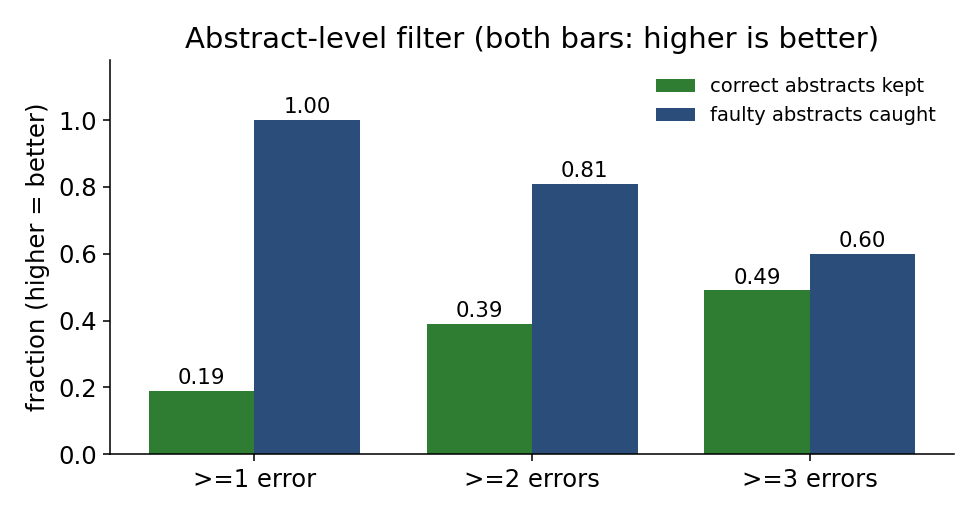
\includegraphics[width=\linewidth]{figures/abstract_level.png}
    \end{column}
  \end{columns}
\end{frame}

% ---------------------------------------------------------------- classifier
% \begin{frame}{The relation classifier (\bert{1}, Chris)}
%   \begin{itemize}
%     \item PubMedBERT classifier reproducing the BioRED baseline.
%     \item The paper's F1 is computed unusually: micro-F1 that excludes the
%           \tc{NoRelation} class from positive scoring.
%     \item Recomputed the same way, our classifier is $\approx$\textbf{44\%}, a
%           realistic baseline. We underperform state of the art a bit, but now we have
%           a number to close the gap against.
%   \end{itemize}
% \end{frame}

% ================================================================ BERT 1 part
\begin{frame}[plain]
  \begin{center}
    {\Large\bfseries\color{accent} The Relation Classifier in Detail}\\[0.4em]
    {\normalsize \bert{1}: Pipeline, Training, Results}
  \end{center}
\end{frame}

% ---------------------------------------------------------------- task
\begin{frame}{The Task and the Prompt}
  Same task as the BioRED baseline: Name the \textbf{relation} between two \textbf{entities} that are already linked, with the \textbf{abstract} as context.
  \begin{itemize}
    \item \textbf{9-way} classification problem (8 BioRED relation types plus \tc{NoRelation})
    \item Currently \textbf{one pair} per forward pass% -- the model never sees the other candidate pairs of the abstract.
    % \item Entities go in by concept id, using the longest mention as the surface form.
  \end{itemize}
  \vspace{0.3em}
  \begin{center}
    \fbox{\begin{minipage}{0.92\textwidth}\footnotesize\ttfamily\raggedright
      Relation: hepatocyte nuclear factor (HNF)-6 -> [MASK] -> Type II diabetes mellitus\\
      Context: The transcription factor hepatocyte nuclear factor (HNF)-6 is an upstream regulator of several genes involved in \dots
    \end{minipage}}
  \end{center}
  \vspace{0.2em}
\end{frame}

% ---------------------------------------------------------------- data
\begin{frame}{Building the Training Data}
  The official splits are used. All presented numbers are based on the \textbf{Train} split.

  The \textbf{gold} relations are taken \textbf{as they are}, the negatives we have to build ourselves.

  \pause

  \begin{itemize}
    % \item A candidate is any entity pair co-mentioned in an abstract but not linked by a gold relation.
    \item No relations are generated using \textbf{two entities} that \textbf{appear} in the abstract but are \textbf{not related}.
    \pause
    \item To balance the dataset only a \textbf{subset} of the possible no relations is used.
    \pause
    \item It is \textbf{measured how far} apart \textbf{related} entities are on \tc{Train}\footnote{mean 73.8 characters, median 37.0, max 1{,}599}.
    \pause
    \item Per abstract everything above that maximum is dropped, the rest is \textbf{sorted by closeness} to the mean, and keep as many as the abstract has gold relations.
    \pause
    \item Prevents the model from mostly learning ``far apart $=$ no relation''.
  \end{itemize}
  \vspace{0.2em}
  \pause
  $\rightarrow$ Results in \textbf{8{,}340} entries in the \tc{Train} split, 2{,}323 in \tc{Dev} and 2{,}326 in \tc{Test}.
\end{frame}

% ---------------------------------------------------------------- distribution
% \begin{frame}{The class imbalance}
%   \begin{center}
%   \small
%   \begin{tabular}{lr@{\hspace{1.2em}}l}
%     \toprule
%     class & train rows & \\
%     \midrule
%     \tc{NoRelation}           & 4{,}162 & \cbar{4.00cm}\\
%     \tc{Association}          & 2{,}192 & \cbar{2.11cm}\\
%     \tc{Positive\_Correlation} & 1{,}089 & \cbar{1.05cm}\\
%     \tc{Negative\_Correlation} &   763 & \cbar{0.73cm}\\
%     \tc{Bind}                 &    61 & \cbar{0.06cm}\\
%     \tc{Cotreatment}          &    31 & \cbar{0.03cm}\\
%     \tc{Comparison}           &    28 & \cbar{0.03cm}\\
%     \tc{Drug\_Interaction}     &    11 & \cbar{0.01cm}\\
%     \tc{Conversion}           &     3 & \cbar{0.01cm}\\
%     \bottomrule
%   \end{tabular}
%   \end{center}
%   \vspace{0.2em}
%   {\small \textbf{Four classes hold 98\% of the rows.}
%   The rare ones have single-digit support in the test set -- \tc{Conversion} appears once -- so macro-F1 over nine classes is mostly noise and we do not report it.}
% \end{frame}

% ---------------------------------------------------------------- models
\begin{frame}{Models and Training Setup}
  \begin{columns}[T]
    \begin{column}{0.5\textwidth}
      \textbf{Two encoders, same pipeline:}
      \begin{itemize}\small
        \item \tc{NeuML/pubmedbert-base-embeddings}\\
              12 layers, hidden 768, 30{,}522 word pieces.
        \item \tc{bioformers/bioformer-8L}\\
              8 layers, hidden 512, 32{,}768 word pieces, about a quarter of the compute.
      \end{itemize}
    \end{column}
    \begin{column}{0.5\textwidth}
      \textbf{Hyperparameters:}
      \begin{itemize}\small
        \item 10 epochs, AdamW, weight decay 0.01.
        \item Batch 32 at lr $5\cdot10^{-5}$, halved to 16 at $2.5\cdot10^{-5}$ on the 8\,GB GPU.
        \item fp16 on CUDA, maximum sequence length 512.
        \item One checkpoint per epoch, best one picked on \tc{Dev}, then scored once on \tc{Test}.
      \end{itemize}
    \end{column}
  \end{columns}
  \vspace{1em}
  {A fresh classification head is attached on top of the encoder. The input is cut off at 512 word pieces.}
\end{frame}

% ---------------------------------------------------------------- eval trap
\begin{frame}{Evaluation Real F1 vs BioRED F1}
  The BioRED paper doesnt specifiy which type of f1 score they used.\\
  Micro-F1 over all nine classes was assumed.
  
  Instead it's a special-case micro-F1 that \textbf{ignores} the \tc{NoRelation} class.
  % Our \tc{compute\_metrics} used plain micro-F1 over all nine classes, which \textbf{gives a point for exactly those rows}.
  \vspace{0.3em}
  % \begin{center}
  % \small
  % \begin{tabular}{l|lcc}
  %   \toprule
  %   gold & prediction & BioRED scorer & actual micro-F1\\
  %   \midrule
  %   relation & same relation      & TP        & correct\\
  %   relation & other relation     & FN and FP & wrong\\
  %   relation & \tc{NoRelation}    & FN        & wrong\\
  %   \tc{NoRelation} & relation    & FP        & wrong\\
  %   \tc{NoRelation} & \tc{NoRelation} & \textcolor{warn}{ignored} & \textcolor{warn}{correct}\\
  %   \bottomrule
  % \end{tabular}
  % \end{center}
  % \vspace{0.3em}

  {\small \textbf{The Real f1 results were higher, because we rewarded the ability to say 'no'}.}
\end{frame}

% ---------------------------------------------------------------- results
%
% INTERPRETATION OF THESE NUMBERS (source comment, not shown on the slide)
%
% The three columns answer three different questions and only the last one is honest:
%
%   micro-F1 (9 cls.)    Accuracy over all rows, including a free hit for every pair the
%                        model correctly rejects. Half of the test rows are such pairs and
%                        NoRelation is the easiest class (per-class F1 0.81), so this column
%                        mostly measures how well the model says "no". Not comparable to
%                        anything published.
%
%   BioRED F1            The correct scoring rule (correct rejections score nothing), but on
%                        a test set where every second candidate pair really is a relation.
%                        A document does not look like that. The number is inflated because
%                        precision is measured against 1,163 negatives instead of 8,934.
%
%   BioRED F1, all neg.  Same rule, all 10,097 co-mentioned pairs of the test abstracts.
%                        This is the number to quote and to optimise against.
%
% Why 0.638 must not be read as "we are close to state of the art":
% it is an artefact of the balanced test set we built for training convenience.
% The realistic figure for the same model is 0.399, and even that is flattered by the fact
% that our models were trained at a 1:1 positive/negative ratio while the test set runs at
% roughly 1:7.7, so they over-claim relations.
%
% Evidence that the training ratio is what matters (from the checkpoint step counts in
% eval.ipynb: 261 steps/epoch = 8,340 rows = 1:1 negatives; 969 steps/epoch = ~31,000 rows
% = all negatives):
%   - supervisor run trained at 1:1, scored on all negatives  -> BioRED F1 ~0.32-0.34
%   - our PubMedBERT  trained at 1:1, scored on all negatives -> BioRED F1  0.399
%   - supervisor run trained on all negatives, same test set  -> BioRED F1  0.4375  (the ~44%)
% So training on the realistic negative distribution is worth roughly 4-6 points, and that
% is the first thing to change, not the model or the learning rate.
%
% Smaller observations:
%   - PubMedBERT beats Bioformer-8L in every column; the 8-layer model is not just cheaper,
%     it is genuinely weaker here (0.619 vs 0.530 on the matched set).
%   - Errors are dominated by Association (support 635, F1 0.640) and by confusion between
%     Association and the two correlation types. The four rare classes contribute almost
%     nothing either way (combined support 32 of 1,163).
%   - "Is there a relation at all" is much easier than typing it: binary F1 0.827 on the
%     matched test set versus 0.638 for the typed task.
%
\begin{frame}{All runs, re-scored}


        {\small Models were evaluated on the \textbf{same test set} (original BioRED) and \textbf{same selection rule} (best epoch on \tc{Dev}).}
  \begin{center}
  \small
  
  \setlength{\tabcolsep}{5pt}
  \begin{tabular}{l|lccc}
    \toprule
    model & training data & micro-F1 (9 cls.) & BioRED F1 & BioRED F1, all rels.\\
    \midrule
    % PROVENANCE of every number in this table
    % ----------------------------------------
    % All four rows come from the SAME checkpoints as before; nothing was retrained.
    % The values were produced by reevaluate_biored_metric.py (stored in results.jsonl under
    % "actual_metrics") and were each re-derived independently by the per-epoch sweep
    % epoch_curves.py. All 11 stored values matched the sweep to the last digit, so no number
    % in this table is "new" in the sense of coming from a new training run.
    %
    % TWO THINGS CHANGED versus the previous version of this table.
    %
    % 1. ONE TEST SET. Both rows use the pure-BioRED test split (2,326 matched /
    %    10,097 all rels., 1,163 gold), built by the builder that resolves comma-joined
    %    MeSH ids correctly.
    %
    % 2. ONE SELECTION RULE FOR EVERYONE. Every row is now the checkpoint the training
    %    pipeline itself selected, load_best_model_at_end on Dev micro-F1:
    %      PubMedBERT / BioRED  epoch 8      Bioformer-8L / BioRED  epoch 9
    %    Previously two rows quoted the best-on-TEST checkpoint (epochs 5 and 4), which is
    %    test-set selection and contradicted the "best one picked on Dev" claim on the setup
    %    slide. Dropping it costs about 2 points and buys a defensible protocol:
    %      PubMedBERT   / BioRED  0.638 -> 0.619 matched, 0.399 -> 0.375 all rels.
    %      Bioformer-8L / BioRED  0.548 -> 0.530 matched, 0.314 -> 0.312 all rels.
    %    For reference, the best-on-Test checkpoint would give 0.6383 / 0.3988 (PubMedBERT).
    %
    % Provenance: no model was retrained. All numbers come from finetuning/epoch_curves.csv,
    % produced by finetuning/epoch_curves.py, which scores all 40 checkpoints on both splits.
    % The rows that existed before are reproduced by that sweep to the last digit.
    PubMedBERT   & BioRED           & 0.724 & 0.619 & 0.375\\
    Bioformer-8L & BioRED           & 0.675 & 0.530 & 0.312\\
    \bottomrule
  \end{tabular}
  \end{center}
  \vspace{0.4em}

  \begin{itemize}
    % \item Taking away the free \tc{NoRelation} hits \textbf{costs about 10 points}: 0.724 $\to$ 0.619 for PubMedBERT.
    \item PubMedBERT stays \textbf{ahead} of Bioformer-8L in every column.
    \item Column \textbf{three} evaluates on the \textbf{balanced} test set, \textbf{column four} uses \textbf{every candidate relation} in the abstract.
          
  \end{itemize}
\end{frame}

% ---------------------------------------------------------------- epoch curves
%
% DATA PROVENANCE (source comment, not shown on the slide)
%
% Every checkpoint of all four runs re-scored by finetuning/epoch_curves.py; the figures are
% drawn from finetuning/epoch_curves.csv by finetuning/plot_epoch_curves.py, so they can be
% restyled without touching a GPU. epoch_curves.json additionally holds the per-class scores.
% No model was retrained: the checkpoints are the original ones from 2026-07-01.
%
% What the curves show:
%   - Training is essentially finished after 4-5 epochs. Everything past that is noise of
%     +-0.02, so the remaining 5 epochs buy nothing. Epoch 3 dips in every single run, which
%     is suspicious enough to be worth a look (same seed, same schedule).
%   - The gap between the solid and the dashed line of one colour is the negative-set effect,
%     not a training effect: same checkpoint, same metric, more candidate pairs.
%   - Bioformer-8L on all pairs (red dashed) is flat from the first epoch at ~0.31. It gets
%     better at the balanced task while not improving at all on the realistic one.
%
\begin{frame}{The Same Runs, Epoch by Epoch}
  \vspace{-0.4em}
  \begin{center}
    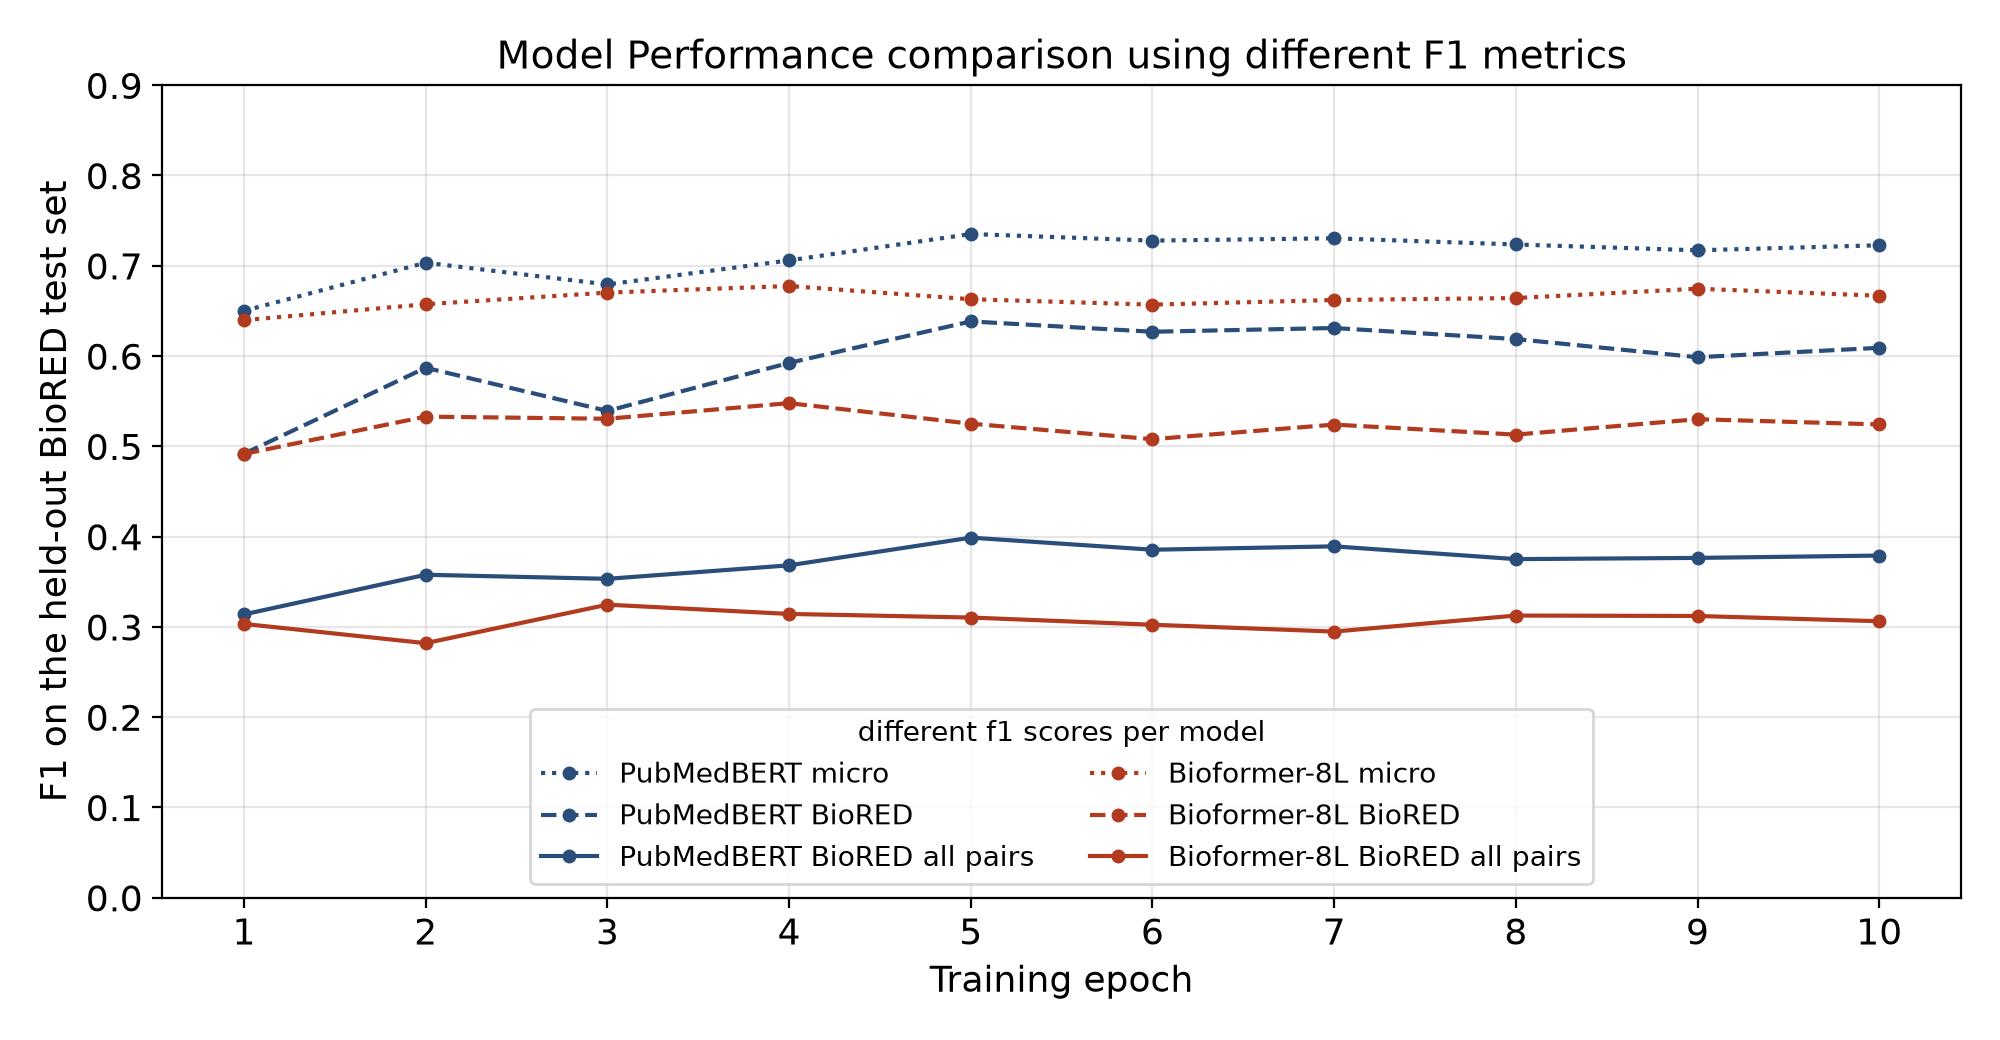
\includegraphics[width=0.80\textwidth]{figures/biored_f1_per_epoch_all_runs_with_micro.png}
  \end{center}
  \vspace{-0.6em}
  {\small \textbf{Nothing learned after epoch 4-5}
  % A solid and its dashed line are the same checkpoints on more candidate pairs.

  All checkpoints were also \textbf{scored on \tc{Dev}} and yielded nearly the \textbf{same} results.
  
  $\rightarrow$ No measureable difference between the splits. No overfitting on checkpoint selection.}
\end{frame}

% ---------------------------------------------------------------- negatives
%
% INTERPRETATION (source comment, not shown on the slide)
%
% The mechanics of the two rows are worth understanding, because they say where the model
% actually fails:
%
%   Recall is identical (0.633) in both rows, and that is not a coincidence: adding negatives
%   cannot change how many true relations the model finds. Recall is a property of the model
%   alone, precision is a property of the model *and* the candidate set it is judged on.
%
%   Precision falls 0.623 -> 0.270. In absolute terms: 715 true positives against 433 false
%   positives on the matched set, against 1,935 on the full set. The decomposition (from
%   negative_discrimination in epoch_curves.json) is:
%       gold-negative rows claimed as a relation :  195 -> 1,697
%       gold rows given the wrong relation type  :  238 ->   238  (same rows, same model)
%   So the model claims a relation on 1,697 of the 8,934 unrelated pairs, 19.0%. Every such
%   pair is a document-level false positive that a real extraction pipeline would emit.
%   These are the Dev-selected checkpoint (epoch 8), matching the results table. The earlier
%   version of this slide quoted epoch 5 (0.638 / 0.399), which was selected on Test.
%
%   Composition of the two test splits (identical positives, only the negatives differ):
%       matched : 2,326 rows = 1,163 gold + 1,163 NoRelation
%       full    : 10,097 rows = 1,163 gold + 8,934 NoRelation
%   The 1,163 gold relations are Association 635, Positive_Correlation 325,
%   Negative_Correlation 171, Cotreatment 14, Bind 9, Comparison 6, Drug_Interaction 2,
%   Conversion 1. TP 736 + FN 427 = 1,163, which is the recall denominator.
%
% Consequence for the project: the QC filter (BERT 2) is aimed at exactly this failure mode,
% a model that claims relations too readily. If filtering the synthetic training data reduces
% the false-positive rate at constant recall, that shows up here as precision, and it is the
% cleanest place to look for an effect.
%
% Caveat on comparing to the ~44%: the supervisor's notebook builds 10,063 rows for the same
% split where we build 10,097 (0.3% difference, presumably the distance cap that we drop when
% all negatives are requested). Close enough to compare, not close enough to call identical.
%
\begin{frame}{Impact of classifiying all relations in an abstract}

  \vspace{0.4em}
  \begin{center}
  \small
  \setlength{\tabcolsep}{4.5pt}
  \begin{tabular}{l|rrrrrr}
    \toprule
    test set (PubMedBERT, BioRED) & entries & real rel. & no-relation & precision & recall & F1\\
    \midrule
    one \tc{NoRelation} per gold relation & 2{,}326 & 1{,}163 & 1{,}163 & 0.623 & 0.615 & 0.619\\
    all co-mentioned pairs              & 10{,}097 & 1{,}163 & 8{,}934 & 0.270 & 0.615 & 0.375\\
    \bottomrule
  \end{tabular}
  \end{center}
  \vspace{0.4em}
  {\small 
  %The 1{,}163 real relations are the same rows in both lines, only the negatives grow.
  %Recall therefore cannot change, extra negatives do not hide a true relation.
  \textbf{Precision more than halves}: the model claims a relation on 1{,}697 of the 8{,}934 unrelated pairs, 19\%.

  \textbf{Recall is unchanged}: \textbf{715} of the \textbf{1{,}163} real relations are classified correctly (61.5\%) in both settings.}

\end{frame}

% ---------------------------------------------------------------- validation
%
% INTERPRETATION (source comment, not shown on the slide)
%
% After the metric mistake, a number is only worth as much as its verification, so both
% directions were checked:
%
%   1. Old metric, new code: the re-scoring script also recomputes the 9-class micro-F1 on
%      the test set it rebuilds. It reproduces the stored value of all seven entries bit for
%      bit (e.g. 0.7351676698194325). That rules out a different test set or a broken
%      model/tokenizer pairing, and isolates the metric as the only change.
%
%   2. New metric, foreign code: eval.ipynb is executed headlessly on our own checkpoint by
%      finetuning/validate_with_eval_notebook.py and prints TP=736, FP=1792, FN=427,
%      P=0.2911, R=0.6328, F1=0.3988, identical to what our script stored. The notebook is
%      not modified on disk; the copy is patched for the absolute /home/flabonte paths, the
%      checkpoint, and Trainer(tokenizer=) -> Trainer(processing_class=), which transformers
%      5.x requires. The scoring functions themselves run unchanged.
%
%   3. The truth table on the "What BioRED counts" slide is not a reading of the scorer but
%      a test of it: finetuning/check_scoring_truth_table.py execs compute_biored_f1 out of
%      eval.ipynb and scores all 9x9 = 81 (gold, prediction) combinations one row at a time.
%      Each combination is mapped to the slide row that claims to cover it, and the row only
%      passes if every combination under it books the same thing. That checks the five rows
%      are correct AND that they leave no case uncovered. It needs no GPU and runs in seconds.
%      The one thing worth flagging when presenting: gold = relation, pred = other relation
%      books FN *and* FP, so a wrong relation type is penalised twice.
%
% What this does and does not prove: the pipeline and the scorer agree, and our numbers are
% reproducible from a second implementation. It says nothing about whether the *setting*
% (which negatives, which split) is the right one; that is a modelling decision, see the
% previous slide.
%
% \begin{frame}{Checking that the numbers hold}
%   We got the metric wrong once, so this time both directions were checked.
%   \begin{itemize}
%     \item \textbf{Old metric, new code.}
%           The re-scoring script also recomputes the 9-class micro-F1 and hits the stored value of all seven runs exactly.
%           So the test set and the model loading are the same as before, and \textbf{the metric really is the only difference}.
%     \item \textbf{New metric, someone else's code.}
%           \tc{eval.ipynb} runs headlessly on one of our checkpoints and prints what our script had stored:
%   \end{itemize}
%   \vspace{0.2em}
%   \begin{center}
%   \small
%   \begin{tabular}{lccccc}
%     \toprule
%      & TP & FP & FN & precision & F1\\
%     \midrule
%     \tc{eval.ipynb} (executed)          & 736 & 1{,}792 & 427 & 0.2911 & 0.3988\\
%     \tc{reevaluate\_biored\_metric.py}  & 736 & 1{,}792 & 427 & 0.2911 & 0.3988\\
%     \multicolumn{6}{l}{\footnotesize (PubMedBERT, \tc{checkpoint-2610}; not the epoch quoted in the results table)}\\
%     \bottomrule
%   \end{tabular}
%   \end{center}
%   \vspace{0.2em}
%   {\small The notebook is not modified on disk.
%   The copy that runs only gets the absolute paths, the checkpoint and one \tc{transformers}\,5 rename.
%   The scoring table two slides back was checked the same way, against all 81 label combinations.
%   All three checks are scripts and can be rerun.}
% \end{frame}

% ---------------------------------------------------------------- issues
\begin{frame}{Failures: Best Off}
  \begin{itemize}
    \item \textbf{Wrong splits.} Final evaluation and epoch evaluation was both done on \tc{Dev}.
    \item \textbf{No saved models.}
          If the models were not explicitly dumped, they were gone.
    \item \textbf{Wrong score.}
          The metric problem from the slide before, which made everything look better than it was.
    \item \textbf{Comparing different results.} Comparing results, created by different test-sets is not clever.
    \item \textbf{Score all relations} Can't just score one \tc{NoRelation} per gold relation, must score all co-mentioned pairs.
    \item \textbf{Forgetting the NoRelation entries.} (:
    \end{itemize}
\end{frame}

% ---------------------------------------------------------------- next steps chris
%
% INTERPRETATION (source comment, not shown on the slide)
%
% Ordering rationale: step 1 is first because it is the only one that changes the baseline
% itself, and every later comparison is measured against that baseline. Training at the
% realistic 1:7.7 negative ratio is worth an estimated 4-6 points (see the results-slide
% comment) and costs nothing but a longer epoch: 31,071 training rows instead of 8,340.
% Doing steps 2-4 before that would mean comparing three conditions against a baseline we
% already know is mis-specified.
%
\begin{frame}{Next steps for \bert{1}}
  \begin{enumerate}
    % \item \textbf{Train on the realistic negative set} instead of the balanced one, and report that number.
    \item \textbf{Synthetic data:} train on the LLM-generated abstracts.
    \item \textbf{Filtered synthetic data:} train on whatever the QC model (\bert{2}) keeps.
    \item \textbf{Compare to the baseline.} See how the model perfomes, based on the different training sets.
    \item \textbf{Bonus:} Find out why we're below the BioRED baseline.
    \item \textbf{Check the abstract-level filter} vs. abstract length and number of
          relations (e.g. make sure it is not only short abstracts passing).
  \end{enumerate}
  \vspace{0.4em}
\end{frame}


% ---------------------------------------------------------------- summary
\begin{frame}{Summary}
  \begin{center}\large Thank you. Questions?\end{center}
\end{frame}

% ---------------------------------------------------------------- bonus
%
% All numbers are the Dev-selected checkpoint of each run (the one the training pipeline
% saved to <run>_dump): PubMedBERT epoch 8, Bioformer-8L epoch 9. Evaluation is the
% all-pairs setting: every co-mentioned entity pair of the 100 Test abstracts, 10,097 rows
% of which 1,163 are real relations. Source: finetuning/epoch_curves.csv and .json.
%
% Reading aids for questions:
%   - FP splits into pairs claimed as a relation that are not one, and real relations given
%     the wrong type. The second kind also books an FN, so a wrong type costs twice.
%   - "Relation vs. none" ignores the type entirely: did the model notice something is there.
%     Both models sit near 0.50, so half of that decision is wrong before typing even starts.
%   - micro-F1 is high only because 88% of the rows are pairs the model correctly rejects.
%
\begin{frame}{Bonus: all numbers, all co-mentioned pairs}
  {\small Scored on all 10{,}097 co-mentioned pairs of the 100 \tc{Test} abstracts: 1{,}163 real relations, 8{,}934 unrelated pairs.}
  \vspace{0.2em}
  \begin{center}
  \scriptsize
  \setlength{\tabcolsep}{6pt}
  \renewcommand{\arraystretch}{0.95}
  \begin{tabular}{lcc}
    \toprule
     & \textbf{PubMedBERT} & \textbf{Bioformer-8L}\\
    \midrule
    checkpoint (best on \tc{Dev}) & epoch 8 & epoch 9\\
    \midrule
    true positives & 715 & 596\\
    false positives & 1{,}935 & 2{,}061\\
    \quad unrelated pair claimed & 1{,}697 & 1{,}761\\
    \quad wrong relation type & 238 & 300\\
    false negatives & 448 & 567\\
    \midrule
    precision & 0.270 & 0.224\\
    recall & 0.615 & 0.513\\
    \textbf{BioRED F1} & \textbf{0.375} & \textbf{0.312}\\
    \midrule
    micro-F1 (9 classes) & 0.788 & 0.769\\
    macro-F1 (9 classes) & 0.392 & 0.259\\
    ``relation vs.\ none'' F1 & 0.500 & 0.469\\
    \midrule
    F1 \tc{Association} ($n$ 635) & 0.341 & 0.285\\
    F1 \tc{Positive\_Corr.} ($n$ 325) / \tc{Negative\_Corr.} ($n$ 171) & 0.409 / 0.419 & 0.376 / 0.312\\
    \bottomrule
  \end{tabular}
  \end{center}
\end{frame}

\end{document}
